%% LyX 2.2.1 created this file.  For more info, see http://www.lyx.org/.
%% Do not edit unless you really know what you are doing.
\documentclass[twocolumn]{IEEEtran}
\usepackage[T1]{fontenc}
\usepackage[latin9]{inputenc}
\usepackage{array}
\usepackage{refstyle}
\usepackage{float}
\usepackage{multirow}
\usepackage{amsmath}
\usepackage{graphicx}
\usepackage[unicode=true,
 bookmarks=false,
 breaklinks=false,pdfborder={0 0 0},pdfborderstyle={},backref=false,colorlinks=false]
 {hyperref}
\hypersetup{pdftitle={Your Title},
 pdfauthor={Your Name},
 pdfpagelayout=OneColumn, pdfnewwindow=true, pdfstartview=XYZ, plainpages=false}
\usepackage{breakurl}

\makeatletter

%%%%%%%%%%%%%%%%%%%%%%%%%%%%%% LyX specific LaTeX commands.

\AtBeginDocument{\providecommand\secref[1]{\ref{sec:#1}}}
\AtBeginDocument{\providecommand\subsecref[1]{\ref{subsec:#1}}}
\AtBeginDocument{\providecommand\tabref[1]{\ref{tab:#1}}}
%% Because html converters don't know tabularnewline
\providecommand{\tabularnewline}{\\}
\RS@ifundefined{subsecref}
  {\newref{subsec}{name = \RSsectxt}}
  {}
\RS@ifundefined{thmref}
  {\def\RSthmtxt{theorem~}\newref{thm}{name = \RSthmtxt}}
  {}
\RS@ifundefined{lemref}
  {\def\RSlemtxt{lemma~}\newref{lem}{name = \RSlemtxt}}
  {}


%%%%%%%%%%%%%%%%%%%%%%%%%%%%%% User specified LaTeX commands.
% for subfigures/subtables
\usepackage[caption=false,font=footnotesize]{subfig}
\renewcommand{\thetable}{\arabic{table}}
%\renewcommand{\figurename}{Fig.}
%\newref{fig}{name = \RSFig.txt}
%\newref{tab}{name = \RSTabtxt}
%\newref{eq}{name = \RSEqtxt}
%\newcommand{\squeezeup}{\vspace{-2.5mm}}

\makeatother

\begin{document}

\title{Ultrafast Transmission Line Fault Detection Using a DWT Based ANN}

\author{Ahmad~Abdullah,~\IEEEmembership{Member,~IEEE} \thanks{Paper previously presented at the 2016 Power and Energy Conference
(PECI), University of Illinois Urabana-Champaign, IL, Feb. 19-20}\thanks{Ahmad Abdullah is with the Department of Electrical Power and Machines,
Faculty of Engineering, Cairo University, Egypt and Electric Power
Engineers Inc., Austin, TX, USA, e-mail: \protect\href{mailto:ahmad.abdullah@cu.edu.eg}{ahmad.abdullah@cu.edu.eg}.}}
\maketitle
\begin{abstract}
Digital impedance protection of transmission lines suffers from known
shortcomings not only as a principle but also as an application as
well. This necessitates developing a new relaying principle that overcomes
those shortcomings. Such a principle is offered in this paper and
is currently being validated using field data. The principle is a
new application of wavelet based artificial neural networks (ANNs).
The application uses high frequency content of a subset of local currents
of one end of a protected line to classify transients on the line
protected and its adjacent lines. The scheme can classify transients
\textendash including faults- occurring on a protected line, categorize
transients on adjacent lines and pinpoint the line causing the transient
event. It is shown that the feature vector of the event can be determined
from a subset of local currents without using any voltages altogether.
The subset of local currents consists of the two aerial modes of the
local current. Modal transformation is used to transform phase currents
to modal quantities. Discrete Wavelet Transform (DWT) is used to extract
high frequency components of the two aerial modal currents. A feature
vector is built using the wavelets details coefficients of one level
of the aerial modes and used to train an artificial neural network.
Results show that the classes corresponding to each transient event
type on the protected line and its adjacent lines are almost linearly
separable from each other. Results demonstrate that very accurate
classification using one eighth of a cycle of post-event data is possible.
\end{abstract}

\begin{IEEEkeywords}
Transmission Line Relaying, Wavelets Transform, Modal Analysis, Artificial
Neural Networks, Power System Faults, Line Switching, Lightning Strike,
Current Transformers
\end{IEEEkeywords}


\section{Introduction\label{sec:Introduction}}

\IEEEPARstart{P}{rotection} of a transmission line involves installing
relays at both ends of the line that constantly monitor voltages and
currents and act when a fault occurs on a line. Traditional protection
uses phasor estimation to estimate the fundamental component of voltages
and currents and take a decision when certain criteria corresponding
to certain fault conditions are met. Distance protection is the most
widely used method for transmission line protection. Modern numerical
distance relays make use of low pass and antialiasing filters - to
reject high frequency content and apply Nyquist sampling theorem-
and special DSP hardware to perform sophisticated math functions \cite{Phadke2009}.
CVTs are generally used to measure the voltages making them available
to the relay. It is known that due to the interaction between the
capacitive voltage divider and the transformer inductance, oscillations
are imposed on the fundamental frequency measured \cite{Kojovic1994}.
This puts more stringent requirement on the filters used in the relay.
Additionally, distance relay can only protect up to 85\% of the line
instantaneously \cite{4113471}. This necessitates the use of a communication
link between the relays at the two ends of the line to achieve fast
tripping from both ends. With relays connected to substation LANs,
a communication link between relays is a cyber-threat. With all limitations
mentioned above, a new relaying principle is needed. This principle
has to be using currents only, fast, and finally does not need any
communication link for its operation. Such a principle is provided
and theoretically tested in this paper. 

Except for traveling wave fault location techniques that are still
not very popular with relay manufacturers \cite{schweitzer2014locating},
little is done with the high frequency components of the transients
even though it has been known that high frequency components of faults
and transient events contain rich information \cite{Santoso1996}.
This is mainly because the traditional mathematical method at hand
was Fast Fourier Transform \cite{Lyons1997}. The FFT requires the
signal be stationary in the wide sense for the calculation of coefficients
to be accurate, i.e., the signal cannot have any temporal variations
for the calculation of coefficients to be correct and accurate. Short
Window Fourier Transform \cite{oppenheim1989discrete} can solve some
of the problems with the FFT but it introduces other issues. However
most signals encountered in power systems are not stationary but have
their characteristics change with time. 

Multiresolution analysis (MRA) is a signal processing tool that has
been introduced in the nineties \cite{Mallat1989} to solve some of
the problems inherent in Fourier transform analysis methods. Wavelets
\cite{daubechies1990wavelet} are usually used along with MRA to solve
this very exact problem. Wavelets have a strong localization property
that enables studying changes not only in time but also in frequency
feasible. It is known from the uncertainty principle \cite{Boggess2009}
that if the signal spans a small portion of the time domain then its
Fourier Transform will span a large portion of frequency domain. The
DWT on the other hand does not suffer from such a limitation. On the
contrary, the signal is approximated at various levels \textendash frequency
bands- and changes in time manifest themselves at the coefficients
of the wavelets only around the time in which the event occurred.
Such property makes it ideal to detect disturbances and study power
system transients \cite{wilkinson1996discrete}. 

With the advent of wavelets, the power system community has seen a
surge in application of wavelets based methods for various power system
problems notably in the area of power system protection- mainly in
transient based protection schemes, transients\textquoteright{} classification
and fault location. The localization property of wavelets makes it
very convenient in locating faults \cite{Magnago1998}. 

The use of artificial neural network for fault classification and
detection has been given in \cite{Dalstein1995,Kezunovic1995,oleskovicz2001complete}
where voltage and current samples are fed directly to the ANN for
fault detection and classification on the protected line. In \cite{Kezunovic1995}
and \cite{Dalstein1995} samples of voltages and currents are used
as a feature vector to train ANN. With the advent of wavelets, special
wavelets transforms are applied to voltage and current waveforms before
they are fed to the ANN for training. In \cite{Silva2006} and \cite{Mao2001},
the DWT is applied to voltages and currents but instead of feeding
the details coefficients to the ANN, entropy (energy) of the signal
is captured and fed instead to the ANN to make fault type classification
between faults on the same transmission line. In \cite{Martin2003}
and \cite{Zwe-Lee2004}, the DWT is applied to voltage and current
signals at a relay location resulting in series of details coefficients
that are fed to the ANN for fault detection and type classification.
In \cite{perera2011recognition} the energy of certain current levels
and approximations is used to train a probabilistic classifier, and
using this energy feature a decision is made whether a transient signal
if due to a fault or non-fault condition on a line. A detailed look
at literature reveals that very few attempts have been done to harness
the power of the wavelets details coefficients alone and understand
their underlying structure. Moreover, existing classification techniques
as the ones in \cite{Zwe-Lee2004} do not take transients on adjacent
lines into account which could mislead these schemes. Additionally,
symmetrical line configuration has been universally assumed which
is a configuration nearly nonexistent in real power systems. 

In this paper, the wavelets details coefficients are directly used
to train the ANN without using any entropy based method. This paper
proposes a novel application for wavelet based ANN. It is shown that
using the details coefficients of a subset local currents only, distinction
can be made between fault and non-fault conditions on a protected
transmission line without using any voltage signals at all. The proposed
algorithm can also distinguish between faults on the protected line
and faults on adjacent lines. The algorithm provided can not only
tell the difference between forward and reverse faults but also can
determine which adjacent line is faulted. It is also shown that the
same apply for lightning strikes and line switching cases, i.e., the
algorithm can tell which line is causing which transient event. Just
as the FFT produces coefficients that correspond to certain frequencies,
wavelets details also give information regarding the oscillatory components
of the signal localizing them in time. In this regard, the DWT is
used to extract useful oscillatory information about the signal. Oscillatory
information is manifested in the wavelets details coefficients at
various levels. It is shown that any transient event on a specific
transmission line causes currents to oscillate in a unique way and
these oscillations can be detected in the wavelets details coefficients
themselves at various levels. The use of these wavelets details coefficients
show the possibility of building ultra-high speed relays. 

The paper is organized as follows: a quick overview of both the DWT
and ANN is offered in \secref{Background}. The rationale behind the
proposed principle is presented in \secref{Rationale-Behind-the}.
The solution methodology is given in \secref{Solution-methodology}.
The simulation platform which consists of a description of EMTP model
and the creation of transient cases for ANN training is described
in \secref{Simulation-Platform}. The structure of the feature vector
is given in \secref{Building-of-Feature}. Signal analysis is provided
in \secref{Signal-Analsysis}. Simulation results are presented in
\secref{Results}. Error analysis is provided in \secref{Error-Analysis}.
Comparison between the method proposed in this paper and existing
methods in literature is offered in \secref{Comparison-to-lit}. Conclusions
and future research are provided at the end of the paper.

\section{Background\label{sec:Background}}

In this section, a brief overview of both the DWT and ANN as used
in this paper is provided. 

\subsection{Discrete Wavelet Transform}

In this paper, the dyadic wavelet transform is used \cite{Boggess2009}.
The transform takes the signal and applies low and high pass filters
to it. The transform converts the original signal into independent
signals each of which spanning a certain frequency band. The frequency
bands are determined by the number of levels the original signal is
sought to be analyzed and each level corresponds to a unique frequency
band. The word independent means that one level cannot be derived
from another, i.e., level 2 cannot be derived from level 1. The frequency
band of each level depends on the sampling frequency and Nyquist theory.
The highest frequency that can be seen in the decomposed signal will
be at most equal to half of the sampling frequency. Given a certain
sampling frequency, the dyadic transform will first apply high and
low pass filters to the signal resulting in two signals. The signal
corresponding to the output of the high pass filter is called level
1 and the other signal is called approximation 1. Both of those signals
are independent. One can stop at this step or can apply high and low
pass filters to the first approximation to get level 2 and approximation
2. Level 2 will span a frequency band corresponding to the upper half
of the frequency band of approximation 1 while approximation 2 will
occupy the lower frequency band. Continuing this manner, by applying
successive low and high pass filters, one obtains a set of levels
-also called details- and one last approximation. In theory, the last
approximation should correspond to a pure sine wave assuming that
the high frequency components imposed on the power frequency have
frequencies that are not included in the frequency band of the last
approximation. Taking a numerical example, if one uses 200 kHz sampling
frequency, then the resulting DWT decomposition is shown in Fig. \ref{fig:DWT-example}.
The details coefficients of the DWT transform is provided in (\ref{eq:DWT_eq})
\cite{Boggess2009} where $\varphi(t)$ is the mother wavelet used,
$f(t)$ is the signal to be analyzed, parameter ``a'' causes scaling
(which determines the level) and ``b'' causes shift in time. In
practice it is not needed to apply the transform all over the infinite
time line. Since wavelets have a strong localization property then
it is only needed to apply the transform to the time period under
study. 
\begin{figure}[h]
\centering{}\includegraphics[scale=0.7]{\string"graphics/DWT flow chart\string".eps}\caption{DWT at 100 kHz sampling rate for 5 levels\label{fig:DWT-example}}
\end{figure}
\begin{equation}
Wf\left(a,b\right)=\frac{1}{\sqrt{a}}\times\int_{-\infty}^{\infty}f\left(t\right)\times\overline{\varphi\left(\frac{t-b}{a}\right)}dt\label{eq:DWT_eq}
\end{equation}


\subsection{Classification with Artificial Neural Networks}

ANN is very well established tool for classification. The classification
done in this paper is not probabilistic but rather deterministic.
The inputs to ANN are vectors in the n-dimensional space, where n
is the size of each input vector, that need to be mapped to another
output vector space. The size of the output vector space is determined
by the number of output classes one wants to map the input vectors
to. In simple terms, this classification can be shown to be carried
out by ANN \cite{Zurada1992}. All ANNs in this paper consist of three
layers: an input layer, a hidden layer and output layer. Each layer
consists of a certain number of neurons. The connections between those
neurons are called synapses. The input layer consists of junctions
that represent the input. The number of junctions must equal to ``n''
which is the dimension of the input vector. The hidden layer can consist
of any number of neurons. The classification accuracy is greatly affected
by the number of neurons in the hidden layer. The output layer consists
of neurons each of which is activated by a function. The inputs to
this function come from the hidden layer. Classes or more specifically
output classes are the patterns one wants to map the input to. The
main idea behind ANN classification is that if the inputs belong to
linearly separable regions of the n-dimensional space then using ANN,
one can draw hyperplanes in that space so that the space between those
hyperplanes contain only one region and each region is then mapped
to one of the output classes using the activation function in the
output neuron. The weights or more specifically synaptic weights of
the synapses are adjusted during the training phase such that the
vector space is divided into regions each of which corresponds to
a certain class. Any output neuron receives the input vector through
synaptic weights. The resultant is then applied to the function of
the neuron that has the form $g(x)=0$ which is an equation of the
hyperplanes in the n-dimensional space. The function $g(x)=0$ is
realized in the ANN by the neurons and the synaptic weights. The output
of the neuron is activated only if $g(x)$ is positive for the corresponding
input vector. In this paper, the author uses the widely known backward
propagation algorithm for the calculation of weights. Knowledge is
stored in the ANN through those weights. Supervised learning only
is done in this paper. The algorithm of the steepest gradient is used
throughout the paper \cite{Zurada1992}.

\section{Rationale Behind the Proposed Method\label{sec:Rationale-Behind-the}}

When a fault or any transient event occurs, it launches a traveling
wave as well as high frequency oscillatory components. Traveling waves
can be easily quantified as they arrive at the line terminals but
the high frequency oscillatory components cannot. The reason for the
oscillatory components not being easily quantified before in literature
will be explained below. 

At this point, the author needs to introduce new terminology. Speaking
of a certain transmission line, the author calls a fault on that line
a fault case. A fault case has its parameters. Those parameters are:
incipient angle, fault resistance, fault type and fault location.
Thus, a certain fault case on a specific transmission line causes
voltages and currents to oscillate in a manner in accordance with
the parameters of that fault case. The formal solution of the currents
and voltages of a single phase line is given by equations (\ref{eq:1})
and (\ref{eq:2}) (called telegrapher equations) \cite{Grainger1994}

\begin{equation}
\frac{\partial V}{\partial x}=R\times I+L\times\frac{\partial I}{\partial t}\label{eq:1}
\end{equation}
\begin{equation}
\frac{\partial I}{\partial x}=G\times V+C\times\frac{\partial V}{\partial t}\label{eq:2}
\end{equation}

Where: 
\begin{itemize}
\item $I$ and $V$ are the current and the voltage anywhere on the line
\item $R$ and $G$ is the resistance and conductance per unit length of
the line
\item $L$ and $C$ are inductance and capacitance of the line per unit
length
\item $x$ is the distance from a zero reference frame generally taken to
be at either end of the line.
\end{itemize}
A general closed form solution of (\ref{eq:1}) and (\ref{eq:2})
is hard and generally impossible as it depends on the boundary and
initial conditions of the case involved. Perhaps the most straightforward
solution method is to obtain the solution in terms of an infinite
time series expansion. Using infinite time series expansion would
mystify the solution, because the author\textquoteright s intention
is to analyze the frequency content of the signal as this content
changes over time. Application of Laplace and Fourier transforms to
those equations produces integrals that yet to be solved formally.
Moreover, when a three phase line is studied, the above equations
become six equations (two equations for each phase: a voltage and
current equation). Thus, decoupling them is hard undertaking if not
impossible in most cases. If we have mutual coupling between two lines
sharing the same tower, then we have three more equations making them
a total of nine equations. Bearing in mind that those nine equations
are for one line only, those equations then need to be solved simultaneously
along with all other equations in the system. For today power systems
which consist of thousands of lines, solving all equations analytically
in a closed form is behind human ingenuity. 

The main aim is to detect the fault once it is initiated. It is very
apparent that the high frequency fault generated transients are different
for each fault case on a specific line. This is because each fault
case on a specific line has its set of equations as given in (\ref{eq:1})
and (\ref{eq:2}) with unique boundary (lines connected to it) and
initial conditions. Moreover, the same fault case on different lines
will cause different fault generated transients because each case
has its own boundary and initial conditions, which is different for
all neighboring lines. For this reason, no attempt is made to solve
the equations formally but solve them numerically by running EMTP
simulations, extracting the high frequency content then analyzing
them. 

Since the author argues that those frequencies -which change over
time- are different for each line, the author only needs to see the
aggregate of all those frequency components for each line. If intuition
is true then the aggregate of those fault generated high frequencies
will be different for each line. What remains is to investigate how
the feature space can be defined such that this difference can be
attained and this is done in \secref{Building-of-Feature}. If it
is possible to map those frequency components to an n-dimensional
space, then faults corresponding to a certain line should be separable
from faults on adjacent lines. The author takes this idea further
and investigates whether the aggregate of all faults from each line
is actually linearly separable \cite{Zurada1992} from each other.
This is the main argument behind the use of ANN as pattern recognition
approach. 

For any fault occurring on a transmission line, the transient generated
frequency components depend on the initial and the boundary conditions
(the lines connected to the faulted line). Since by definition all
adjacent lines are different then the frequency generated transients
for faults on each transmission line should be unique for each line.
The question is whether those frequency components can be combined
in a certain way to form a pattern to be recognized. 

The same argument not only applies to faults but also apply to switching
events and lightning strikes on transmission lines. The transient
event types that are studied in this paper are faults, lightning strikes,
and line switching. Evidently, the frequency content of faults \textendash on
all lines- should be different from switching which in turn different
from lightning because the equations governing the solutions are always
different as different transient event types have different boundary
and initial conditions. Those events types can be first recognized
and then the event can be traced back to the line originating it as
given in \subsecref{Transient-Event-Type}. This basically means that
there is a mapping that can divide a certain subspace to linearly
separable regions that correspond to those event types. If one zooms
in that event subspace, one can see which line is causing that event
type. 

\section{Solution methodology\label{sec:Solution-methodology}}

In this paper it is argued and shown that the oscillatory information
present in the transient signal captured at a single relay location
caused by sudden network topology changes contains sufficient information
for classification not only between transients on the same line but
also between transients on adjacent lines. Any change of configuration
on the line causes a traveling wave to be generated traveling from
the point of change towards the ends of the line. In the simplest
case this wave will be just a pulse -a step- but in reality will be
accompanied by high frequency oscillating components. Fourier analysis
is not suitable for analyzing such waveforms because those oscillations
will be distorted and attenuated as they arrive at the line terminals.
However, applying the DWT will enable us to see both the spectral
and temporal variations of those high frequency oscillations. 

Historical treatment of traveling waves - as used in the ladder diagram
for example- treat them as if they were pulses traveling down the
line with no regard to the oscillatory components they carry. A certain
mathematical entity -which is the feature vector to be defined in
\secref{Building-of-Feature}- is derived from the oscillatory components
and called the transient signature of the event. The transients that
are studied in this paper are lightning, line switching and faults.
At a certain terminal of the line which is typically a relay location,
it is argued and shown that those signatures are unique to the event
that originated them and to the line which initiated those events.
This means that using this oscillatory information of the event, the
line causing it can be determined. Those signatures are a function
of the line parameters, the network topology and the instance of the
event and, of course, the type of the event. In essence, the signature
of the fault occurring on a certain line will be different form the
signature of the fault on adjacent lines. Also, line switching will
cause the currents to oscillate in a manner that is different from
faults and lightning striking the same line and those oscillatory
components are different for different lines as well.

It is argued that the aggregate of all transient signatures caused
by a certain transient event \textendash switching or faults for example-
originating from a certain line occupies a specific subspace in the
n-dimensional space. This subspace is almost linearly separable \cite{Zurada1992}
from all other subspaces generated by other transient events by adjacent
lines. The n-dimensional space is the space spanned by all n-dimensional
feature vectors used to train the ANN. A relay that is programmed
to use these wavelets details not only can detect and classify transients
on a protected line but also can detect faults and classify transients
on adjacent lines. ANN classification is used to show that this is
indeed the case. Static feedforward ANN is a tool used to map a vector
from the n-dimensional space to another m-dimensional space. In the
case at hand, the feature vector is mapped which is n-dimensional
space to another output space. These output spaces will be described
in \secref{Results}, but for now if this mapping is successful then
the original n-dimensional subspaces are linearly separable as explained
in \cite{Zurada1992}.

Information is extracted from the high frequency components using
the DWT at various levels. Before the DWT is applied, phase currents
are decoupled from each other using modal analysis \cite{Hedman1965,Hedman1965b}.
Modal transformation will decouple current waveforms thus eliminating
mutual coupling and untransposed line effects. The modal matrix will
be explained in \secref{Building-of-Feature}. It is known that CVT
introduces transients to the measured voltage signal. It is shown
in \cite{hou1996capacitive} that a typical CVT with active ferroresonance
suppression circuit is a low pass filter with a cut off frequency
around 1 kHz which drops to almost 200 Hz when passive ferroresonance
suppression circuit is employed. On the other hand classification
with currents is preferable because the cut off frequency of current
transformers is much larger than the potential transformer or CVT.
The useful passband of current transformers is typically 100 kHz \cite{lee1994development}
and in some cases can go up to 400 kHz \cite{Douglass1981a} or 500
kHz \cite{redfern2003laboratory}. Since a conservative stance is
chosen, the sampling rate is selected such that the maximum frequency
available in the signal is 100 kHz to attain the 100 kHz passband
of current transformers. The time step used in the EMTP simulations
is 1$\mu s$ which should theoretically give a maximum frequency of
500 kHz in sampled output according to Nyquist theory. However, it
is given in \cite{Siqueira2015} that the maximum frequency in the
EMTP simulations is only one fifth of that, so the maximum frequency
is 100 kHz.

After decoupling phase quantities, the DWT is applied to the currents
modes to convert the signals to a series of coefficients that will
be used for training of the neural networks. The event is detected
once a change of level 3 -or any level depending on which level is
used- coefficients is detected. This detection is simply because the
pre-event data is assumed steady state so no high frequency components
exist in the pre-event data. Once the event is detected, a window
of one eighth of a cycle of post event information is used for neural
network training. Simulations show that at least one eighth of a cycle
of post-event data has to be used for correct classification. Numerous
trials have shown that at least one eighth of a cycle of post-event
information has to be present for correct classification or classification
fails completely. 

The outcome of the DWT is a series of coefficients for each mode and
for each level. The coefficients of one level of the two aerial modes
of currents are stacked on top of each other to build one feature
vector that will be used to train the network. Building the training
vector will be explained in \secref{Building-of-Feature}. A neural
network of an appropriate size is then selected for classification.
The choice of the size of network is reached at by trial and error
and no universal size has been applied to all classification problems.
That is the size of the network is changed till the required classification
accuracy is achieved. Once the size of ANN is selected, the ANN is
then trained using various scenarios for transients on lines. It is
shown that using only two modes of local current information at one
end of the line - corresponding to a relay, distinction can be made
between various transient events on different lines. It is argued
and shown that the feature vector built has sufficient information
to distinguish between a fault and non-fault condition on a protected
transmission line. It is also shown that the adjacent line causing
certain transient events can be determined. This means using local
information we can see what is happening on adjacent lines.

In summary, the procedure is as follows: 
\begin{enumerate}
\item Decouple currents using modal analysis.
\item Apply the DWT to the aerial modes using one eighth of a cycle of post
event currents.
\item Stack the series of coefficients of the two aerial modes of a certain
level on top of each other to create a vector used to train ANN.
\item A neural network of appropriate size is used for training. Training
is done using transient scenarios. Those scenarios include: faults,
line switching and lightning.
\end{enumerate}

\section{Simulation Platform\label{sec:Simulation-Platform}}

In this section, the ATP/EMTP model is presented in \subsecref{EMTP-Model}
while in \subsecref{Creation-Of-Transient} creation of the transient
cases for the training, validation and testing of ANN is fully described. 

\subsection{EMTP Model\label{subsec:EMTP-Model}}

The area under study is shown in Fig. \ref{fig:fig_1}. The IEEE 118
bus is used \cite{WashStatUni} as a test system. All data is taken
from \cite{WashStatUni} except for machine data and the lines in
the area under study. The dyanmic data of IEEE 118 bus system is taken
from \cite{7151773}. The line under study is the line connecting
buses 23 and 25 (line 23-25). The selection of this is arbitrary but
this specific line was attractive to the simulations for the reasons
that follow. Line 23-25 is bordered by three lines connected to bus
23 namely: line 23-22, line 23-32 and line 23-24. Line 23-25 is also
connected to line 26-30 via a transformer connecting buses 25 and
26. Line 23-25 is also connected to line 25-27 via bus 27. A synchronous
generator is connected to bus 25 via step up transformer. 
\begin{figure}[h]
\begin{centering}
\includegraphics[scale=0.4]{\string"graphics/System_under study\string".eps}
\par\end{centering}
\caption{Portion of the system under study\label{fig:fig_1}}
\end{figure}

All power transformers have been modeled using ATP Hybrid Transformer
Model according to \cite{cho2002parameter} with typical parameters
provided by ATPDraw. Initial high frequency components are measured
well before CT saturation occurs \cite{Perera2008} and since one
eighth only of post-event data is used, the results of \cite{Perera2008}
apply very well in our case, i.e., no need to model CT saturation
effects. Synchronous machines are modeled using ATP SM-59 except for
excitation and governor controls. This is because only one eighth
of a cycle of post event data is used which is a period much shorter
than modern exciter and governor time constants. 

In the simulations that follows, very general tower configurations
are used for the line under study and its adjacent lines. The line
connecting buses 23 and 25 is given in \cite{gashimov2009transmission}.
The tower configurations for the lines bordering lines 23-25 are taken
from \cite{ALSTOM2002}. All towers are reproduced from \cite{ALSTOM2002}
in the paper for convenience of reader in Fig. \ref{fig:fig2}. All
lines in the study area have been modeled as lines with frequency
dependent parameters with ground return. All other lines have been
modeled as symmetrical (fully transposed) lines with frequency dependent
parameters with no ground wire. 

Current measurement devices are located at terminals 23 and 25. It
should be pointed out as well that no attempt has made to model current
transformers because the maximum frequency available in the simulated
signals is 100 kHz which is typically less than the useful passband
of the CT as given in \cite{lee1994development,Douglass1981a,redfern2003laboratory}. 

It should be pointed out that a surge arrester has been also used
in the simulations. The tool in \cite{jonathanwoodworth2014} is used
to select the characteristic of our surge arrester. Bus capacitance
and transformer stray capacitance have also been accounted for with
values given in \cite{greenwood1991electrical} which are extremely
important in high frequency transient studies. 

\subsection{Creation of Transient Cases and Preparation of Cases for Training
of ANN\label{subsec:Creation-Of-Transient}}

The argument in the paper is that high frequency components of the
currents measured at a local relay not only can detect fault and no
faults condition on a protected line but also can detect fault and
no fault condition on adjacent lines. A large number of simulations
had to be carried out to prove this argument. A very general network
topology with different tower configurations is present. 
\begin{figure}[h]
\centering{}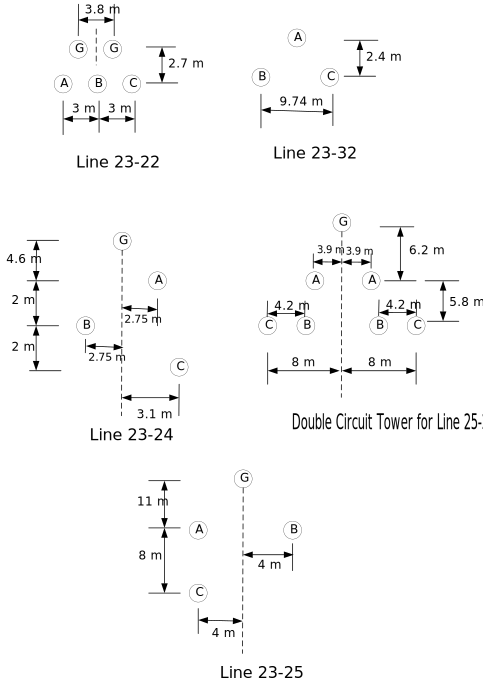
\includegraphics[clip,scale=0.4]{graphics/Tower_Configurations}\caption{Tower Configurations of lines of the area under study \label{fig:fig2}}
\end{figure}

Creation of fault cases, lightning strike cases and line switching
cases has been automated. A toolbox that automatically creates transient
cases is released in \cite{7335090}. Creation of fault cases is first
described then line switching cases and after that the lightning strike
cases. At this point it should be emphasized that the line under study
and that is to be protected is line 23-25 which is bordered by 4 adjacent
lines namely line 23-22, line 23-32, line 23-24, line 25-27. 

No attempt is made to answer how far the local currents can be used
to classify transients on the lines that are beyond the lines directly
connected to the line under study. For this reason, ANN is trained
for the line under study and the five circuits directly surrounding
it only. The next paragraphs describe creation of transient cases
for faults, line switching and lightning and creation of feature vector
for training. 

\subsubsection{Creation of Fault Cases\label{subsec:Creation-of-Fault}}

Fault cases are created in batches; a batch for each line. Each batch
has fault parameters, these parameters are the following: incipient
angle, fault resistance, fault location and fault type. All types
of faults have been created, i.e., AG, BG, CG, AB, BC, CA, ABG, CBG,
ACG, ABC, ABCG. Incipient angles are from 0 to 350 degrees in 10 degrees
increments. Fault resistance assumes the values: 0, 20 $\Omega$,
100 $\Omega$ and 1000 $\Omega$. The distance takes the following
values: 5\%, 15\%, 35\%, 50\%, 65\%, 80\% and 95\% which are all percentages
of total line length. Simulations are created for line 23-25 and it
adjacent lines. 

A total of 8066 cases per batch have been created which gives a total
of 48396 cases because line 25-27 is double circuit line, i.e., two
batches of faults for line 25-27 have been created: one for each circuit.
Fault arc although simulated but was not taken into account during
training. This is because fault arc causes, if any, very little distortion
to phase currents which is consistent with the results in \cite{perera2011recognition}
and \cite{Dalstein1995}. The previous statement has been validated
using the fault arc model given in \cite{Terzija2004}.

\subsubsection{Creation of Line Switching Cases\label{subsec:Creation-of-Line-switching-cases}}

For line switching cases, a batch for each line has been created giving
a total of 6 batches. Each batch consists of smaller batches; each
of the smaller batches corresponds to switching by one of the circuits
breakers at each terminal. For example, line 23-22 would have a smaller
batch for switching using the breaker installed on terminal 23 and
another smaller batch for switching using the breaker on terminal
22. The variable in switching cases is the moment of switching. Switching
times ranges from 0 to 360 degrees in 2 degrees increment. This way
360 cases per batch have been created, giving a total of 2160 cases.

\subsubsection{Creation of Lightning Strike Cases\label{subsec:Creation-of-Lightning-cases}}

For lightning strike cases, a batch of each line has been again created.
An ATP Heidler type lightning source with rising time equal to 4 $\mu s$
and a $\tau$ equal to 10 $\mu s$ has been used. The rising and tailing
times are kept constant during simulations but amplitudes have been
varied which were set to 5 kA, 10 kA, 15 kA, 20 kA and 30 kA. Striking
distances were the same as the ones used for fault batches: 5\%, 15\%,
35\%, 50\%, 65\%, 80\% and 95\% which are all percentages of total
line length. The incipient angle was 0, 90,180, 270 and 330 degrees.
This amounts to 630 cases per batch giving a total of 3780 cases. 

\section{Building of Feature Vector of Transient Signature\label{sec:Building-of-Feature}}

After batches have been created, a special subroutine is used to translate
the phase quantities to modal quantities. The phase quantities are
decoupled using the modal matrix calculated at 10 kHz even though
the matrix is frequency dependent. Different modal frequencies for
the modal matrix have been tried but this did not affect the classification
results at all. The two aerial modes are the only ones used for training.
The modal matrix with real entries is given in (\ref{eq:eq4}). The
signs of the entries are only shown to emphasize their physical meaning
\begin{equation}
\begin{pmatrix}Mode1\\
Mode2\\
Mode3
\end{pmatrix}=\begin{pmatrix}+ & + & +\\
- & + & +\\
+ & + & -
\end{pmatrix}\times\begin{pmatrix}Ia\\
Ib\\
Ic
\end{pmatrix}\label{eq:eq4}
\end{equation}

It should be apparent that Mode1 is the weighted sum of all phase
currents which is nothing other than the ground mode current. This
ground mode current is known to be very well dependent on the frequency
and ground resistance on the contrary to the aerial modes that are
more or less frequency independent \cite{Ametani2013}. This is the
main reason that the ground current mode has not been used for building
the feature vector for training. 

Once the modal quantities are available, we run the DWT with db4 for
4 levels, starting from level 1 to level 4. Db4 has been used since
it has produced good results with previous literature. The outcome
of the DWT is a series of coefficients for each level and for each
mode. Since the first one eighth of a cycle following the transient
event is only sought, the details coefficients corresponding to that
period are only obtained. Two modes out of the three modes are only
used. The details coefficients of one level of Mode2 and Mode3 are
stacked on top of each other. It should be emphasized that building
the n-dimensional vector this way does not change the temporal content
of the feature vector, as long as all other n-dimensional vectors
are built consistently this way, i.e., the order of the modes in the
feature vector has to be preserved and the vector has to be built
using one level only. If the order of modes in the feature vector
is changed, this amounts to a rotation of n-dimensional space but
should not change the results of classification, again as long as
all vectors are built consistently. 

At this point one should note that the application uses only two thirds
of modes of the currents as contrasted to other applications that
use all phase voltage and current waveforms for ANN training \cite{Martin2003}
which amounts to drastic reduction in computational power needed for
ANN. 

Having created n-dimensional vectors, the input for the ANN is ready.
Training of the ANN is then started. The cases are randomly divided
into the following categories: 70\% of all cases for training, 15\%
for validation and another 15\% for testing.

\section{Signal Analysis\label{sec:Signal-Analsysis}}

Even though ANN training is done offline, yet the principle proposed
in this paper can be used for online applications. It should be noted
that training has been done using hundreds of thousands of cases.
For example, 8066 fault cases per line and a total of 54336 transient
cases have been used to train ANN as given in \subsecref{Creation-Of-Transient}.
These cases encompass all variations of any transient that can occur
on a transmission line. ATP/EMTP is mature enough that it can capture
the actual system response. A real event oscillography would look
like the simulated case in EMTP as long as the EMTP model is an accurate
representation of the system. It is not possible to exhaust all foreseen
transient parameters, for example it is not computationally feasible
to include all values of fault resistance into consideration in the
training stage. However, it is evident that the oscillations present
in the transient signal corresponding to a fault case with a fault
resistance of 20 $\Omega$ should have oscillations that fall in between
the same fault case but with a fault resistance of 0 $\Omega$ and
100 $\Omega$. This notion of \textquotedblleft in-betweenness\textquotedblright{}
is illustrated in Fig. \ref{fig:fault_resistance}. As explained in
\secref{Solution-methodology}, the transient signal is eventually
translated into a vector that belongs to the n-dimensional space.
Thus if the fault cases corresponding to 5\%, 20\%, 80\% and 95\%
line length can be linearly separated from all other transients, then
the fault cases corresponding to 50\% line length should fall in the
region of those fault cases. The same argument applies for all event
types. This idea of \textquotedblleft in-betweenness\textquotedblright{}
makes this approach applicable to online applications as long as the
extreme cases are included in the offline training. 

\section{Results\label{sec:Results}}

This section presents the results of the classification. In \subsecref{LINE-IDENTIFICATION-IN-faults},
the results of classification in case all events were faults are shown.
In \subsecref{Line-Identification-in-switching} results in case events
were all line switching are presented. In \subsecref{Line-Identification-in-lightning}
classification output in case of all events were lightning strikes
is shown. Finally, event type classification is provided in \subsecref{Transient-Event-Type}. 

In \secref{Solution-methodology}, the mapping from n-dimensional
space to the m-dimensional space has not been discussed. The dimension
of the n-dimensional space is fixed by the length of the feature vector
while the dimension of the m-dimensional space varies according to
which space we want to map the n-dimensional space to. In \subsecref{LINE-IDENTIFICATION-IN-faults},
\subsecref{Line-Identification-in-switching} and \subsecref{Line-Identification-in-lightning}
below, the events are being mapped to the lines causing them 
\begin{figure}[H]
\centering{}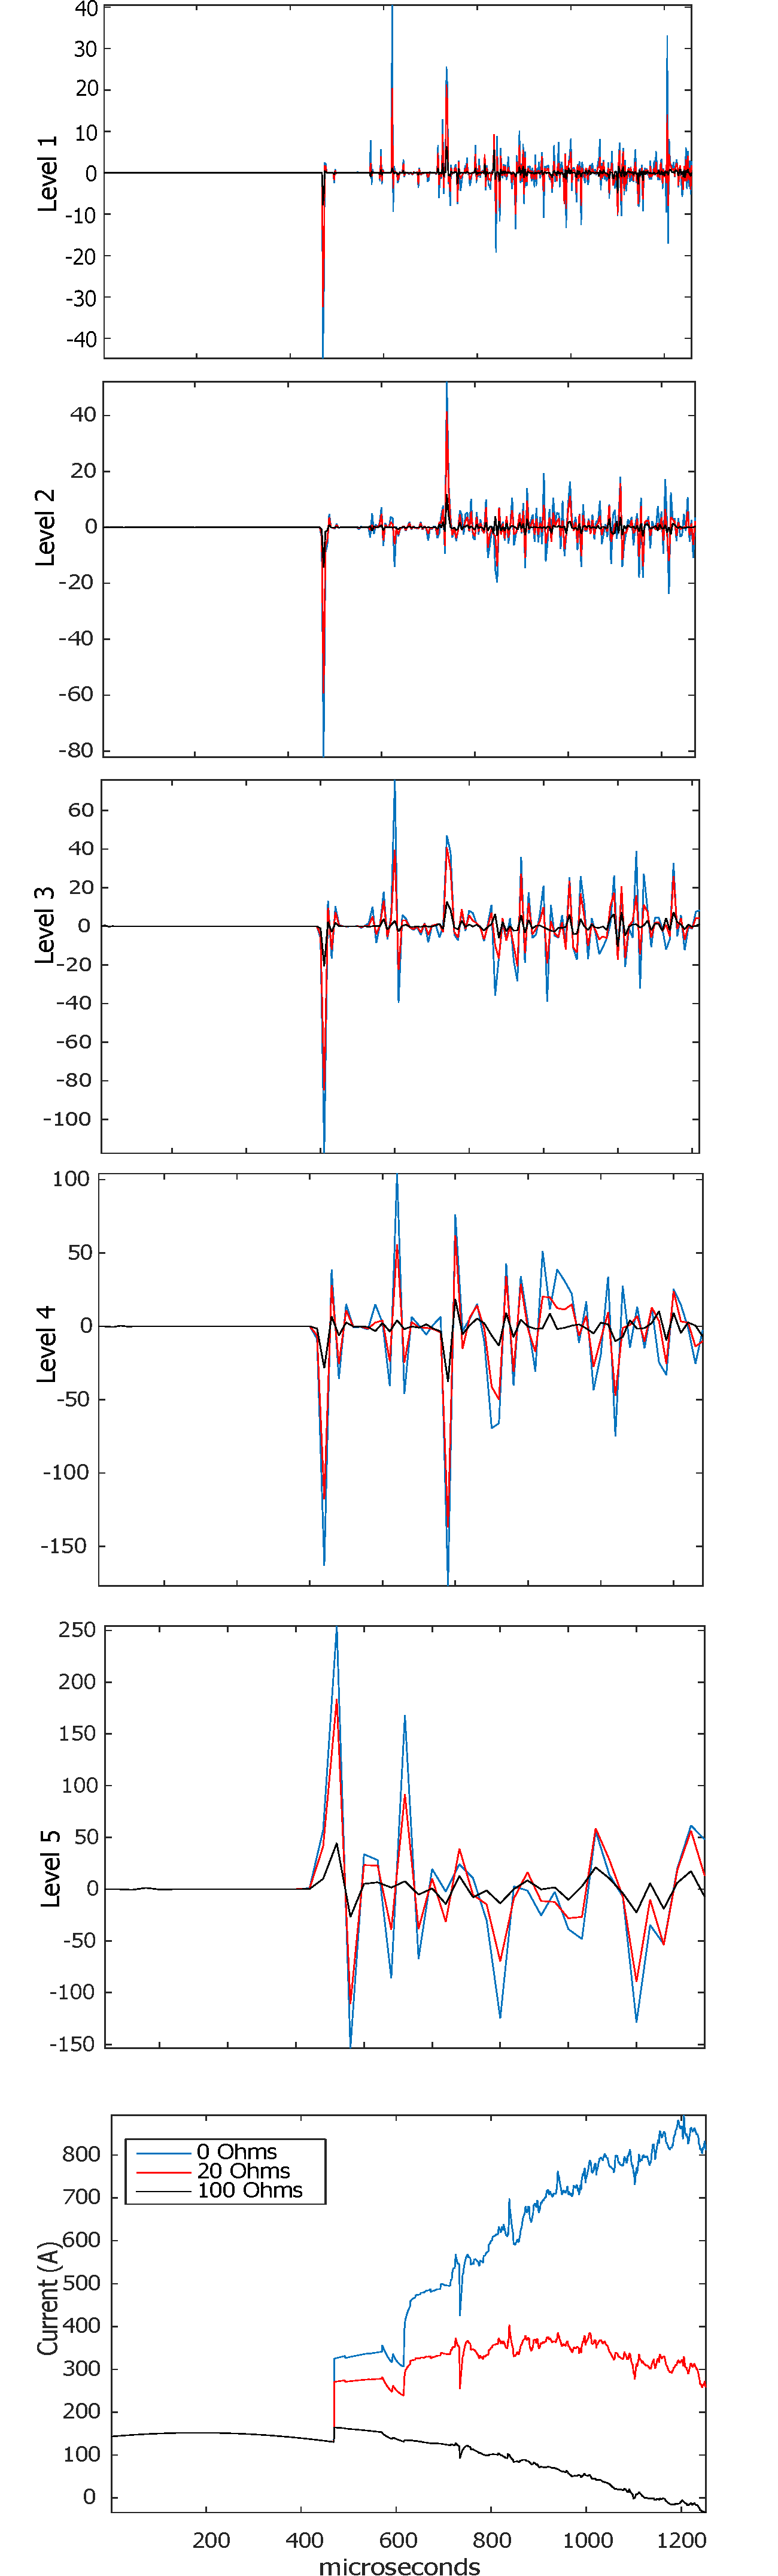
\includegraphics[scale=0.3]{graphics/sigAnalysis}\caption{Mode2 current of a certain fault case at different fault resistances.
The same fault type, fault location and incipient angle is evaluated
but at different fault resistances\label{fig:fault_resistance}}
\end{figure}
 which amounts to a mapping from the n-dimensional space to a 6-dimesnioal
space (one dimension per line, line 25-27 counted twice for the double
circuit). In \subsecref{Transient-Event-Type}, all events are being
mapped to an event-type space which is a mapping from n-dimensional
space to a 3-dimsnsional space (faults, lightning and switching).
It should be apparent that the dimension of the feature space (n-dimensional
space) depends on the DWT level used. It should be obvious as well
that this dimension is almost halved as we go one level higher, i.e.,
the dimension of the n-dimensional space using level 1 is double the
dimension of level 2 n-dimensional. 

\subsection{Line Identification in Case of Faults \label{subsec:LINE-IDENTIFICATION-IN-faults}}

This section provides the results for classification in case all transients
were of faults. 

First, six batches of faults are created as described in \subsecref{Creation-of-Fault}.
Creating the feature vector using currents from terminal 23 as described
before using any levels from 1 to 4 to train ANN gives the classification
accuracy in Table \ref{tab:table1}. One immediately sees that classification
accuracy for the double circuits of line 25-27 fails. This is to be
expected if the reader consults Fig. \ref{fig:fig2} for the tower
configuration which shows that from the Thevenin\textquoteright s
point of view at the terminal 23 or 25 of the line under study, the
same fault case on any circuit will produce the same response due
to the symmetry of the tower 25-27. It should be pointed out that
the faults on one of the circuits of line 25-27 are confused for faults
on the other circuit and vice versa but not with other lines. The
percentage accuracy does not change if the currents at terminal 25
are used instead. Training with levels 1, 2, 3 and 4 gives the same
classification accuracy but the difference is mainly in the ANN size
needed. For reproducibility purposes, an ANN of size 40 in the hidden
layer is needed to achieve the results in Table \ref{tab:table1}
for level 3. Lower levels (levels corresponding to higher frequencies)
needed less neurons but the feature vector becomes so long (corresponding
to more detailed time resolution). This in turn demands for a high
super computer which has been undertaken for level 1 (frequency band
from 100 kHz to 50 kHz) and level 2 (50 kHz to 25 kHz). Level 3 (25
kHz to 12.5 kHz) and level 4 (12.5 kHz to 6.25 kHz) can be done on
a PC such as the one the author used with Core i7, 3.2 GHz speed,
4 cores and 8 GB of RAM. If the double circuit tower 25-27 is considered
to be one line, a 100\% correct classification is achieved for faults.
\begin{table}[h]
\centering{}\caption{Faults Classification Accuracy \label{tab:table1}}
\begin{tabular}{|c|c|}
\hline 
Transmission Line & Accuracy (\%)\tabularnewline
\hline 
Line Under Study & 100\tabularnewline
\hline 
Line 23-32 & 100\tabularnewline
\hline 
Line 23-24 & 100\tabularnewline
\hline 
Line 23-22 & 100\tabularnewline
\hline 
Circuit (1) Line 25-27 & 46\tabularnewline
\hline 
Circuit (2) Line 25-27 & 54\tabularnewline
\hline 
\end{tabular}
\end{table}


\subsection{Line Identification in Case of Switching\label{subsec:Line-Identification-in-switching}}

This section shows the results of classification if all transients
are for line switching. Creating the switching events as described
in \subsecref{Creation-of-Line-switching-cases} and using either
end currents, the accuracy in Table \ref{tab:table2} is achieved.
Training with any level from 1 to 4 gives the same classification
result, but the only difference is being the size of the hidden layer.
Level 3 required 30 neurons in the hidden layer with lower levels
requiring less neurons and higher levels requiring more neurons. Once
again switching events on one of the circuits of line 25-27 are confused
for the other circuit and vice versa.

\subsection{Line Identification in Case of Lightning Strikes\label{subsec:Line-Identification-in-lightning}}

If all transient events are lightning only as described in \subsecref{Creation-of-Lightning-cases},
then using any end data gives the results in Table \ref{tab:table3}
irrespective of the terminal used or the level used (levels 1 to 4).
Level 3 required 30 neurons in the hidden layer with lower levels
requiring less neurons and higher levels requiring more neurons. One
has to note that in Table \ref{tab:table2} and Table \ref{tab:table3},
the algorithm cannot still distinguish between the events on any of
the circuits of line 25-27 due to the symmetry with respect to the
line being studied.
\begin{table}[h]
\caption{Switching Classification Accuracy \label{tab:table2}}

\centering{}%
\begin{tabular}{|c|c|}
\hline 
Transmission Line	 & Accuracy (\%)\tabularnewline
\hline 
Line Under Study & 100\tabularnewline
\hline 
Line 23-32 & 100\tabularnewline
\hline 
Line 23-24 & 100\tabularnewline
\hline 
Line 23-22 & 100\tabularnewline
\hline 
Circuit (1) Line 25-27 & 48\tabularnewline
\hline 
Circuit (2) Line 25-27 & 52\tabularnewline
\hline 
\end{tabular}
\end{table}
 
\begin{table}[h]
\caption{Lightning Classification Accuracy\label{tab:table3}}

\centering{}%
\begin{tabular}{|c|c|}
\hline 
Transmission Line	 & Accuracy (\%)\tabularnewline
\hline 
Line Under Study & 100\tabularnewline
\hline 
Line 23-32 & 100\tabularnewline
\hline 
Line 23-24 & 100\tabularnewline
\hline 
Line 23-22 & 100\tabularnewline
\hline 
Circuit (1) Line 25-27 & 49\tabularnewline
\hline 
Circuit (2) Line 25-27 & 51\tabularnewline
\hline 
\end{tabular}
\end{table}


\subsection{Transient Event Type Classification\label{subsec:Transient-Event-Type}}

Lastly, the algorithm performance is shown when it comes to classification
between different transients types. The types of studies in this paper
are faults, line switching and lightning. ANN is trained with all
transient cases given in \subsecref{Creation-of-Fault}, \subsecref{Creation-of-Line-switching-cases}
and \subsecref{Creation-of-Lightning-cases} above. The output is
shown in Table \ref{tab:table4}. Once again levels 1 through 4 give
the same classification accuracy whether bus 23 or 25 is used. The
ANN used for Table \ref{tab:table4} has a size of 30 when trained
with level 3 currents. It should be pointed out that in Table \ref{tab:table4}
most lightning strikes with amplitude 5000 Amp on line 23-22 have
been misclassified for faults. A 5000 Amp lightning strike is unlikely
in real world lightning strike cases. If we remove all 5000 Amp strikes
from training, a one hundred percent accurate classification is achieved
for event type classification.

It is now a straightforward manner to construct a two layer feedforward
network that classify any event to fault, lightning or switching in
the first layer then identify the line causing the event in the second
layer. Alternatively, a relay can be programmed to classify the events
into fault, switching or lightning per Table \ref{tab:table4}. Once
this is done, the same event can be applied to the ANN corresponding
to that event type.
\begin{table}[h]
\begin{centering}
\caption{Transient Event Type Classification Accuracy \label{tab:table4}}
\par\end{centering}
\centering{}%
\begin{tabular}{|c|c|}
\hline 
Event Type & Accuracy (\%)\tabularnewline
\hline 
Faults & 100\tabularnewline
\hline 
Lightning & 97.2\tabularnewline
\hline 
Switching & 99.8\tabularnewline
\hline 
\end{tabular}
\end{table}


\section{Error Analysis \label{sec:Error-Analysis}}

Since power systems are subject to harsh environmental conditions,
error always exists in the measurements regardless of the bandwidth
of the measuring devices used. The author analyzed the performance
of the proposed algorithm when noise exists in the current measurements.
Noise has been added to the data that has been generated in \subsecref{Creation-Of-Transient}.
The noise that has been added is Gaussian white noise at different
signal-to-noise ratios. The noisy data was then applied to the ANNs
trained in \subsecref{LINE-IDENTIFICATION-IN-faults}, \subsecref{Line-Identification-in-switching},
\subsecref{Line-Identification-in-lightning} and \subsecref{Transient-Event-Type}
to see how noise affects the classification accuracy. As can be seen
from Table \ref{tab:table8}, Table \ref{tab:table9}, Table \ref{tab:table10}
and Table \ref{tab:table11}, classification accuracy decreases as
SNR decreases. Even in the best case with high SNR, classification
accuracy is not as good as it were in \subsecref{LINE-IDENTIFICATION-IN-faults},
\subsecref{Line-Identification-in-switching}, \subsecref{Line-Identification-in-lightning}
and \subsecref{Transient-Event-Type}. This may be because ANN has
bad generalization capability which could signal that a better classification
approach is needed.
\begin{table}[h]
\centering{}\caption{testing ANN in \tabref{table1} with noisy and denoised data in case
of faults \label{tab:table8}}
\begin{tabular}{|c|c|c|c|}
\hline 
\multirow{2}{*}{SNR} & \multirow{2}{*}{Transmission Line} & \multicolumn{2}{c|}{Classification Accuracy}\tabularnewline
\cline{3-4} 
 &  & Noisy Data (\%) & Denoised Data (\%)\tabularnewline
\hline 
\multirow{6}{*}{60} & Line Under Study & 99 & 99.3\tabularnewline
\cline{2-4} 
 & Line 23-32 & 98.2 & 98.7\tabularnewline
\cline{2-4} 
 & Line 23-24 & 98.4 & 99.1\tabularnewline
\cline{2-4} 
 & Line 23-22 & 98 & 98.6\tabularnewline
\cline{2-4} 
 & Circuit (1) Line 25-27 & 48.1 & 48.9\tabularnewline
\cline{2-4} 
 & Circuit (2) Line 25-27 & 49 & 49.4\tabularnewline
\hline 
\multirow{6}{*}{40} & Line Under Study & 96 & 98.2\tabularnewline
\cline{2-4} 
 & Line 23-32 & 95.2 & 97.2\tabularnewline
\cline{2-4} 
 & Line 23-24 & 94 & 98\tabularnewline
\cline{2-4} 
 & Line 23-22 & 93.1 & 97.1\tabularnewline
\cline{2-4} 
 & Circuit (1) Line 25-27 & 46 & 47\tabularnewline
\cline{2-4} 
 & Circuit (2) Line 25-27 & 47 & 48.3\tabularnewline
\hline 
\multirow{6}{*}{30} & Line Under Study & 90 & 97.3\tabularnewline
\cline{2-4} 
 & Line 23-32 & 89 & 96.5\tabularnewline
\cline{2-4} 
 & Line 23-24 & 89 & 96.8\tabularnewline
\cline{2-4} 
 & Line 23-22 & 88.7 & 97\tabularnewline
\cline{2-4} 
 & Circuit (1) Line 25-27 & 42 & 46.5\tabularnewline
\cline{2-4} 
 & Circuit (2) Line 25-27 & 44 & 47.9\tabularnewline
\hline 
\end{tabular}
\end{table}
\begin{table}[h]
\centering{}\caption{testing ANN in \tabref{table2} with noisy and denoised data in case
of switching\label{tab:table9}}
\begin{tabular}{|c|c|c|c|}
\hline 
\multirow{2}{*}{SNR} & \multirow{2}{*}{Transmission Line} & \multicolumn{2}{c|}{Classification Accuracy}\tabularnewline
\cline{3-4} 
 &  & Noisy Data (\%) & Denoised Data (\%)\tabularnewline
\hline 
\multirow{6}{*}{60} & Line Under Study & 98 & 99\tabularnewline
\cline{2-4} 
 & Line 23-32 & 97 & 98\tabularnewline
\cline{2-4} 
 & Line 23-24 & 97.1 & 98\tabularnewline
\cline{2-4} 
 & Line 23-22 & 97.5 & 98.5\tabularnewline
\cline{2-4} 
 & Circuit (1) Line 25-27 & 47.5 & 49.2\tabularnewline
\cline{2-4} 
 & Circuit (2) Line 25-27 & 48.8 & 49.5\tabularnewline
\hline 
\multirow{6}{*}{40} & Line Under Study & 95 & 98\tabularnewline
\cline{2-4} 
 & Line 23-32 & 94.6 & 97.5\tabularnewline
\cline{2-4} 
 & Line 23-24 & 93.5 & 97.2\tabularnewline
\cline{2-4} 
 & Line 23-22 & 92.5 & 98\tabularnewline
\cline{2-4} 
 & Circuit (1) Line 25-27 & 45.5 & 48.7\tabularnewline
\cline{2-4} 
 & Circuit (2) Line 25-27 & 46.1 & 49\tabularnewline
\hline 
\multirow{6}{*}{30} & Line Under Study & 87 & 96.5\tabularnewline
\cline{2-4} 
 & Line 23-32 & 86 & 95.2\tabularnewline
\cline{2-4} 
 & Line 23-24 & 86.2 & 95.6\tabularnewline
\cline{2-4} 
 & Line 23-22 & 87.4 & 96\tabularnewline
\cline{2-4} 
 & Circuit (1) Line 25-27 & 42.2 & 47.6\tabularnewline
\cline{2-4} 
 & Circuit (2) Line 25-27 & 43.5 & 48.5\tabularnewline
\hline 
\end{tabular}
\end{table}
\begin{table}[h]
\centering{}\caption{testing ANN in \tabref{table3} with noisy and denoised data in case
of lightning\label{tab:table10}}
\begin{tabular}{|c|c|c|c|}
\hline 
\multirow{2}{*}{SNR} & \multirow{2}{*}{Transmission Line} & \multicolumn{2}{c|}{Classification Accuracy}\tabularnewline
\cline{3-4} 
 &  & Noisy Data (\%) & Denoised Data (\%)\tabularnewline
\hline 
\multirow{6}{*}{60} & Line Under Study & 100 & 100\tabularnewline
\cline{2-4} 
 & Line 23-32 & 99 & 99.3\tabularnewline
\cline{2-4} 
 & Line 23-24 & 99.1 & 99.5\tabularnewline
\cline{2-4} 
 & Line 23-22 & 99.7 & 99.7\tabularnewline
\cline{2-4} 
 & Circuit (1) Line 25-27 & 49.3 & 49.3\tabularnewline
\cline{2-4} 
 & Circuit (2) Line 25-27 & 49.5 & 49.5\tabularnewline
\hline 
\multirow{6}{*}{40} & Line Under Study & 98 & 99\tabularnewline
\cline{2-4} 
 & Line 23-32 & 97 & 97.8\tabularnewline
\cline{2-4} 
 & Line 23-24 & 97.2 & 98\tabularnewline
\cline{2-4} 
 & Line 23-22 & 97.9 & 98.5\tabularnewline
\cline{2-4} 
 & Circuit (1) Line 25-27 & 46 & 47.3\tabularnewline
\cline{2-4} 
 & Circuit (2) Line 25-27 & 47 & 48.5\tabularnewline
\hline 
\multirow{6}{*}{30} & Line Under Study & 95 & 98\tabularnewline
\cline{2-4} 
 & Line 23-32 & 94 & 96.7\tabularnewline
\cline{2-4} 
 & Line 23-24 & 94.6 & 96.2\tabularnewline
\cline{2-4} 
 & Line 23-22 & 94.8 & 97.6\tabularnewline
\cline{2-4} 
 & Circuit (1) Line 25-27 & 42 & 46.6\tabularnewline
\cline{2-4} 
 & Circuit (2) Line 25-27 & 41.5 & 48.1\tabularnewline
\hline 
\end{tabular}
\end{table}
\begin{table}[h]
\begin{centering}
\caption{testing ANN in \tabref{table4} with noisy and denoised data in case
of all transient events \label{tab:table11}}
\par\end{centering}
\centering{}%
\begin{tabular}{|c|c|c|c|}
\hline 
\multirow{2}{*}{SNR} & \multirow{2}{*}{Event Type} & \multicolumn{2}{c|}{Classification Accuracy}\tabularnewline
\cline{3-4} 
 &  & Noisy Data (\%) & Denoised Data (\%)\tabularnewline
\hline 
\multirow{3}{*}{60} & Faults & 99 & 99.2\tabularnewline
\cline{2-4} 
 & Lightning & 96 & 96.8\tabularnewline
\cline{2-4} 
 & Switching & 98.1 & 98.5\tabularnewline
\hline 
\multirow{3}{*}{40} & Faults & 97 & 98.1\tabularnewline
\cline{2-4} 
 & Lightning & 95.2 & 95.7\tabularnewline
\cline{2-4} 
 & Switching & 96.5 & 97\tabularnewline
\hline 
\multirow{3}{*}{30} & Faults & 95 & 97.5\tabularnewline
\cline{2-4} 
 & Lightning & 94.4 & 95\tabularnewline
\cline{2-4} 
 & Switching & 94.1 & 96.5\tabularnewline
\hline 
\end{tabular}
\end{table}

To remove noise from data, the author used wavelet denoising approach.
The wavelets toolbox in MATLAB has been used to perform wavelet denoising.
The denoised data are used for testing the ANNs trained in \subsecref{LINE-IDENTIFICATION-IN-faults},
\subsecref{Line-Identification-in-switching}, \subsecref{Line-Identification-in-lightning}
and \subsecref{Transient-Event-Type}. The waveform of mode2 current
of a certain fault case with noise (SNR=40) and after denoising is
shown in Fig. \ref{fig:Noisy-Singal}. The results of this testing
is provided in Table \ref{tab:table8}, Table \ref{tab:table9}, Table
\ref{tab:table10} and Table \ref{tab:table11}. As can be seen from
the tables, denoising improves the performance of ANN. This is more
noticeable when classification is done using data that has lower SNR.
A detailed error analysis is beyond the scope of this paper and will
be undertook along with field validation. 
\begin{figure}[h]
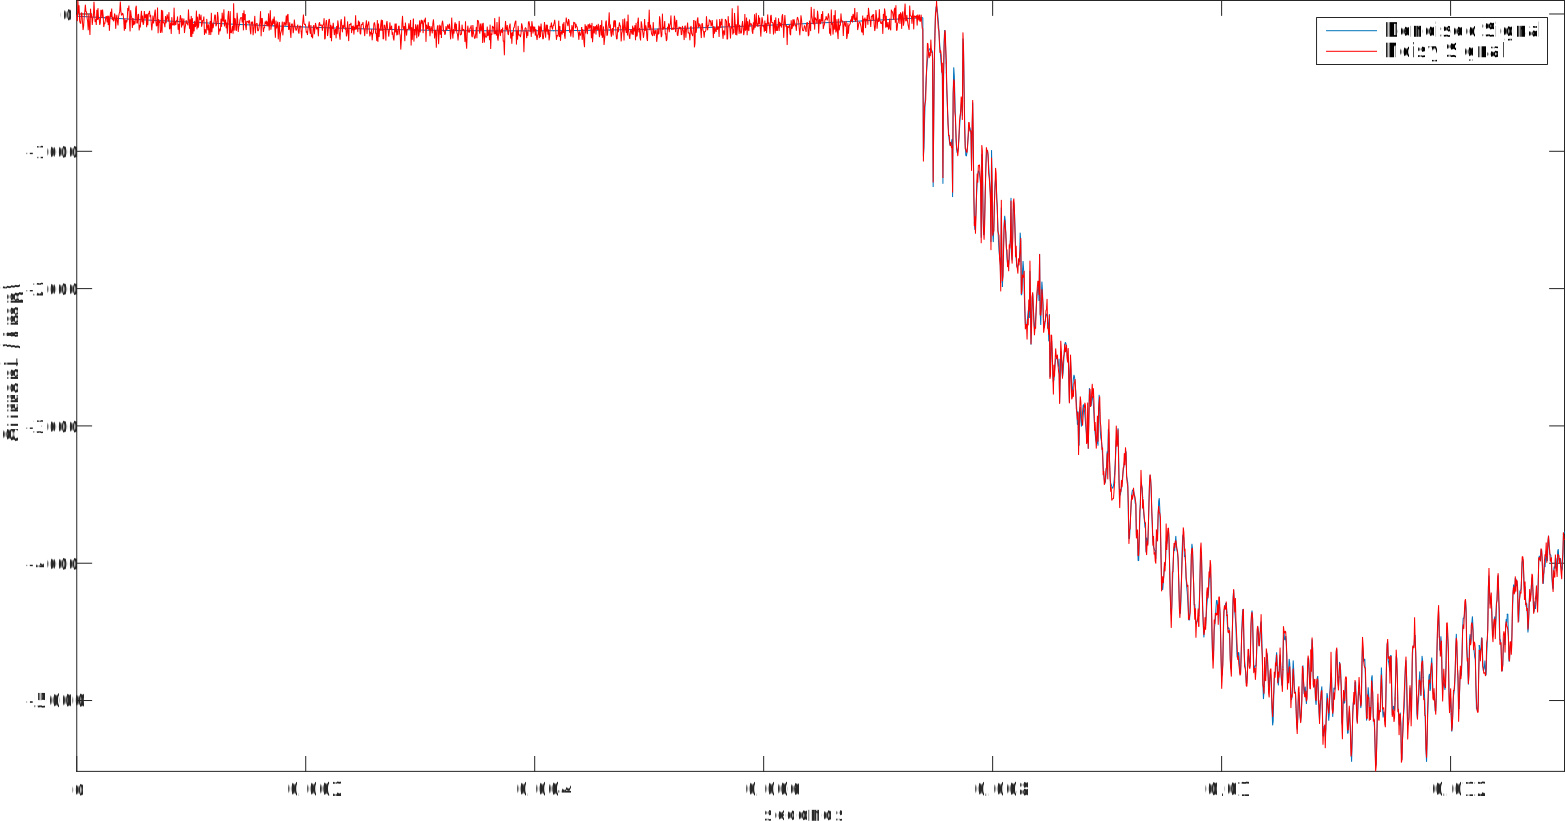
\includegraphics[scale=0.15]{graphics/noise_denoised_signal}\caption{Mode2 of a fault case with noise and after denoising \label{fig:Noisy-Singal} }
\end{figure}


\section{Comparison to Existing Methods in Literature\label{sec:Comparison-to-lit}}

The major drawbacks of existing methods have been summarized in \secref{Introduction}.
In this section, the method proposed will be compared to existing
methods in literature that uses single end data to reach a decision
regarding the fault. 

Even though the subject of transmission line relaying based on high
frequency components has and continues to receive attention from academia
and the industry, a handful of papers studies transients other than
faults and their effect on the proposed methods. 

In \cite{Martin2003}, the details coefficients of all phase voltages
and currents are fed to ANN for training. However, for the method
to perform well, the high frequency transients imposed on the fundamental
voltage have to be measured, which is not feasible if CVTs are used
as the bandwidth of CVTs do not exceed 1 kHz \cite{hou1996capacitive}.
Additionally, the method ignores all transients types other than faults
which can mislead the scheme most of the times. 

In \cite{Silva2006}, the details coefficients of all phase voltages
and currents are still used to train the ANN in addition to using
an energy quantity as a trip restraint. However, transients on the
line being protected are being taken into consideration while training
the ANN. A drawback of this method is the need to perform many offline
studies to determine the threshold for the trip restraint. Moreover,
the method suffers from the limited bandwidth of the CVTs. 

In \cite{perera2011recognition}, the energy of the three phase currents
are used to train a probabilistic classier. Voltages have been abandoned
for the purpose of classification due to the aforementioned shortcomings
of CVTs. However, the simulated system is small and the methods proposed
cannot identify the line causing the transient event. Additionally,
the use of energy as a feature requires a detailed study on the proximity
of the transient to the measuring CT. The results in \cite{perera2011recognition}
is a special case of the results in this paper and correspond to the
results in \subsecref{Transient-Event-Type}. 

For the purpose of statistical comparison, the author has reproduced
the PNN classifier given in \cite{perera2011recognition} and applied
it to the system in Fig. \ref{fig:fig_1}. The training data set that
had been developed in \subsecref{Creation-Of-Transient} is then applied
to the to PNN classifier. The results of classification are provided
in Table \ref{tab:table5}. As can be seen from both Table \ref{tab:table4}
and Table \ref{tab:table5}, not all lightning strikes are fully recognized.
This occurs because some lightning strikes are confused for faults.
The ones that are confused for faults are the ones that have 5 kA
amplitude which is consistent with the observation in \subsecref{Transient-Event-Type}.
Moreover, some faults are not well recognized using the PNN due to
high resistance faults which is consistent with the observation in
\cite{perera2011recognition}. The main advantage of the method given
in this paper is that less features are needed to obtain satisfactory
classification accuracy. 
\begin{table}[h]
\begin{centering}
\caption{PNN Classification Accuracy \label{tab:table5}}
\par\end{centering}
\centering{}%
\begin{tabular}{|c|c|}
\hline 
Event Type & Accuracy (\%)\tabularnewline
\hline 
Faults & 98\tabularnewline
\hline 
Lightning & 96\tabularnewline
\hline 
Switching & 100\tabularnewline
\hline 
\end{tabular}
\end{table}
 

In all methods mentioned above, at least one quarter of a cycle is
needed to reach a secure decision. On the other hand, the approach
proposed in this paper uses only one half of that to reach a secure
decision about whether the transient belongs to the line being protected
and whether the transient is a fault. Additionally, actual physical
tower configurations have not been taken into consideration in literature. 

\section{Conclusions and Future Research}

This paper presented an argument that high frequency signals can be
used for high speed power system fault detection via transient classification
identifying the line causing the transient event. 

The contributions of the paper are as follows: 
\begin{enumerate}
\item It has been shown that currents alone can be used for transient signature
of the event. 
\item Only two modes are necessary for classification. 
\item Only one eighth of a cycle of post event data is necessary for classification. 
\end{enumerate}
Although the results in this paper have been shown only to a specific
tower, the author has tried different tower configurations and confirmed
that the algorithm works for all tower configurations considered.
It should be clear that the current method fails if a lightning strike
evolves to a fault. This drawback has been addressed separately in
a different publication \cite{AbdullahLightn16}. Additionally, detection
of faults on mutually coupled lines has not been addressed in this
paper and will be treated in a different publication.

One issue that has not been investigated in this paper is insulation
breakdown. The author has not assumed any failure of insulation in
the simulations. The cutting of the signal associated with insulation
breakdown can potentially mislead the scheme proposed. Further investigations
are needed to completely quantify its effect on the proposed relaying
scheme. It should be noted, however, that lightning strikes are being
chopped by the surge arrester but still being correctly recognized. 

Field validation is being performed and results will be shared once
all investigations are done.

\section*{Acknowledgment}

This paper could not have seen the light without the resources at
Texas A\&M Supercomputing Facility. The author would like to thank
all at the facility for their help and support. The author also would
like to express his sincere thanks for Jonathan Woodworth of ArresterWorks
for his guidance regarding arrester selection. Lastly, the author
would like to thank Gurunath Gurrala from the Indian Institute of
Science for his constructive review of the manuscript. 

\bibliographystyle{IEEEtran}
\bibliography{references}

\begin{IEEEbiography}[{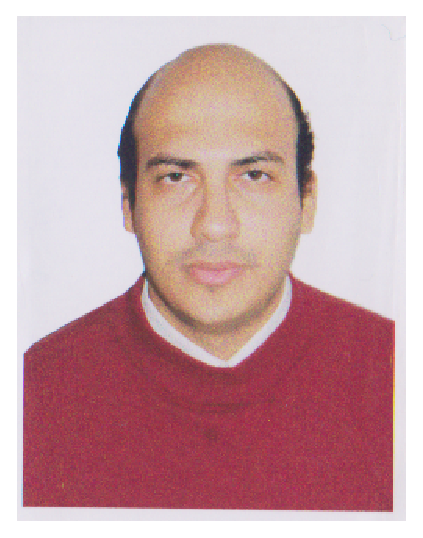
\includegraphics[scale=0.4]{graphics/Pic1}}]{Ahmad Abdullah}
 received his B.Sc. M.Sc. degrees from the Department of Electrical
Power and Machines at the Faculty of Engineering at Cairo University,
Gizah, Egypt, in 2009 and 2012, respectively. He received his Ph.D.
degree from Electrical and Computer Engineering Department at Texas
A\&M University, College Station, TX in 2017. Since 2015, he has been
with Electric Power Engineers, Inc as a power systems engineer responsible
for conducting power system design studies.
\end{IEEEbiography}


\end{document}
